\begin{frame}[t]{Die Messbruecke - mit KTY81} 
    
    \begin{spacing}{0.9} \begin{tiny}
      \begin{table}[h!]
      \begin{tabular}{p{5cm} p{5cm} }
        \hline
        \textbf{Schaltungsaufbau} \\
        \hline \\
        \begin{minipage}{0.5\textwidth}
            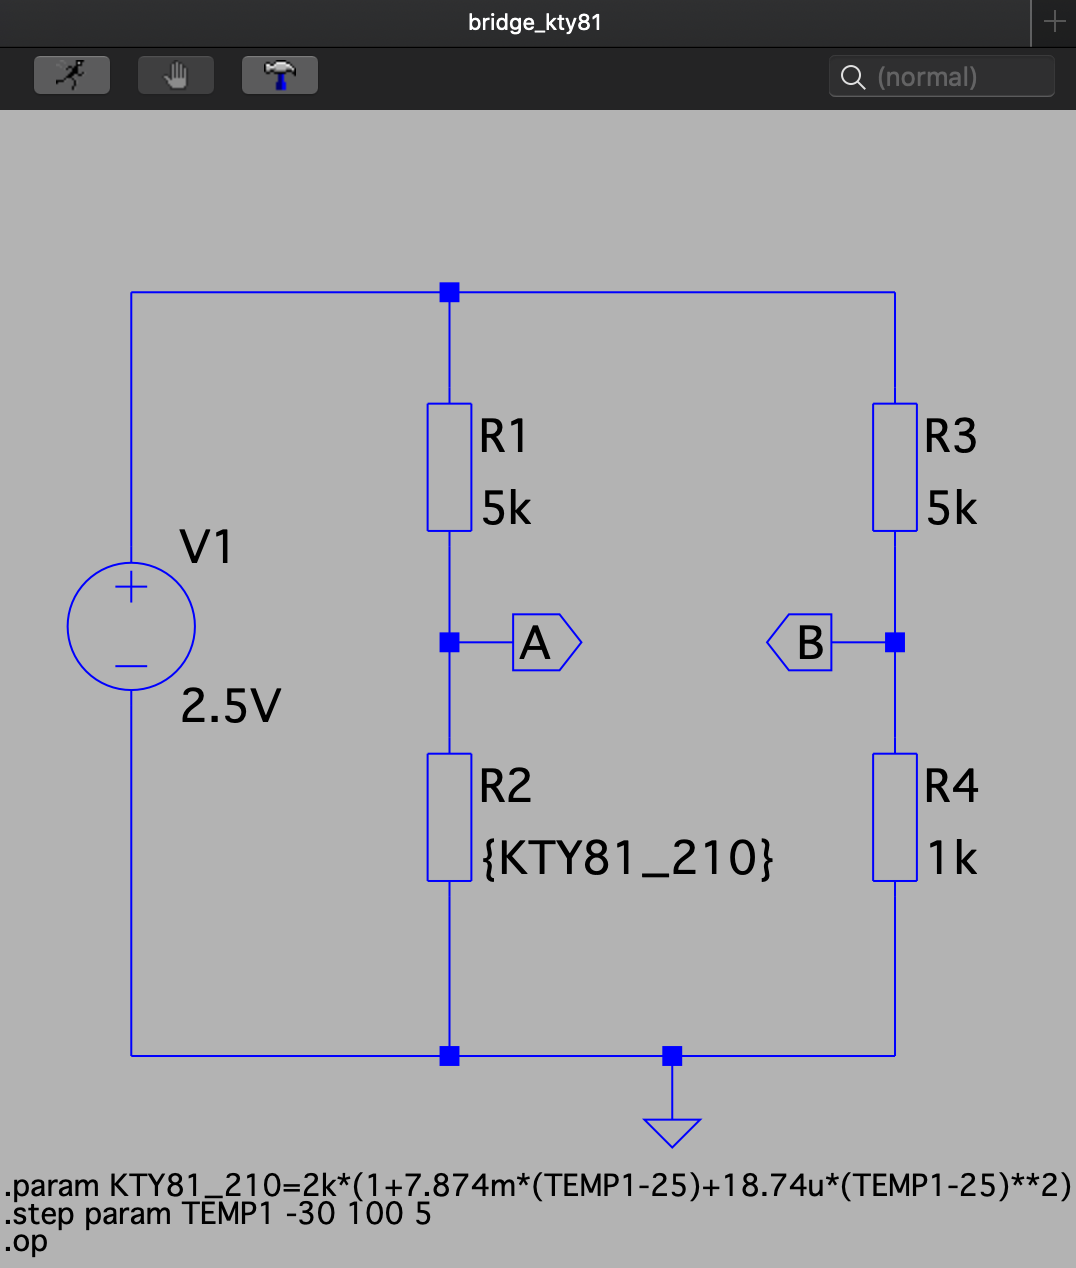
\includegraphics[width=0.9\linewidth]{pictures/mb_kty81.png}
        \end{minipage} 
        &
        \begin{minipage}{0.5\textwidth}
            \begin{itemize}
                \item Ihr baut den KTY81-210 inklusive der als spice-Direktive modellierten Formel in eure Messbreuckenschaltung ein
                \item Prüft ob das Model immer noch simulierbar ist und es zu keinem Fehler kommt. 
            \end{itemize}
        \end{minipage} 
        \\
        
    \end{tabular}

    \end{table}
     
    \end{tiny} \end{spacing}

\end{frame}

\begin{frame}[t]{Die Messbruecke - Linearisierung der Kennlinie} 
    
    \begin{spacing}{0.9} \begin{tiny}
      \begin{table}[h!]
      \begin{tabular}{p{10cm} }
        \hline
        \textbf{Problemstellung} \\
        \hline \\
        \begin{minipage}{\textwidth}
            \begin{itemize}
                \item Die Formel zur Approximation des PTC is quadratisch
                \item Dadruch sind wird unsere Messung "nicht-linear" und wir werden bei einer \textbf{konstanten Temperaturerhöhrung keine
                konstante Spannungserhöhrung} erwarten können
            \end{itemize}
        \end{minipage}  
       \\ \\
       \hline
       \textbf{Simulatives Experiment} \\
       \hline \\
       \begin{minipage}{\textwidth}
       Zur Annäherung werden wir die Vorwiderstand R1 ebenfalls variieren, um experimentell einen linearen Verlauf der Spannung $V_{AB}$ zu ermitteln.
       \end{minipage}
       \\\\
       \begin{tabular}{p{5cm} p{5cm}}
        \begin{minipage}{0.5\textwidth}

           \begin{figure}
               \centering    
               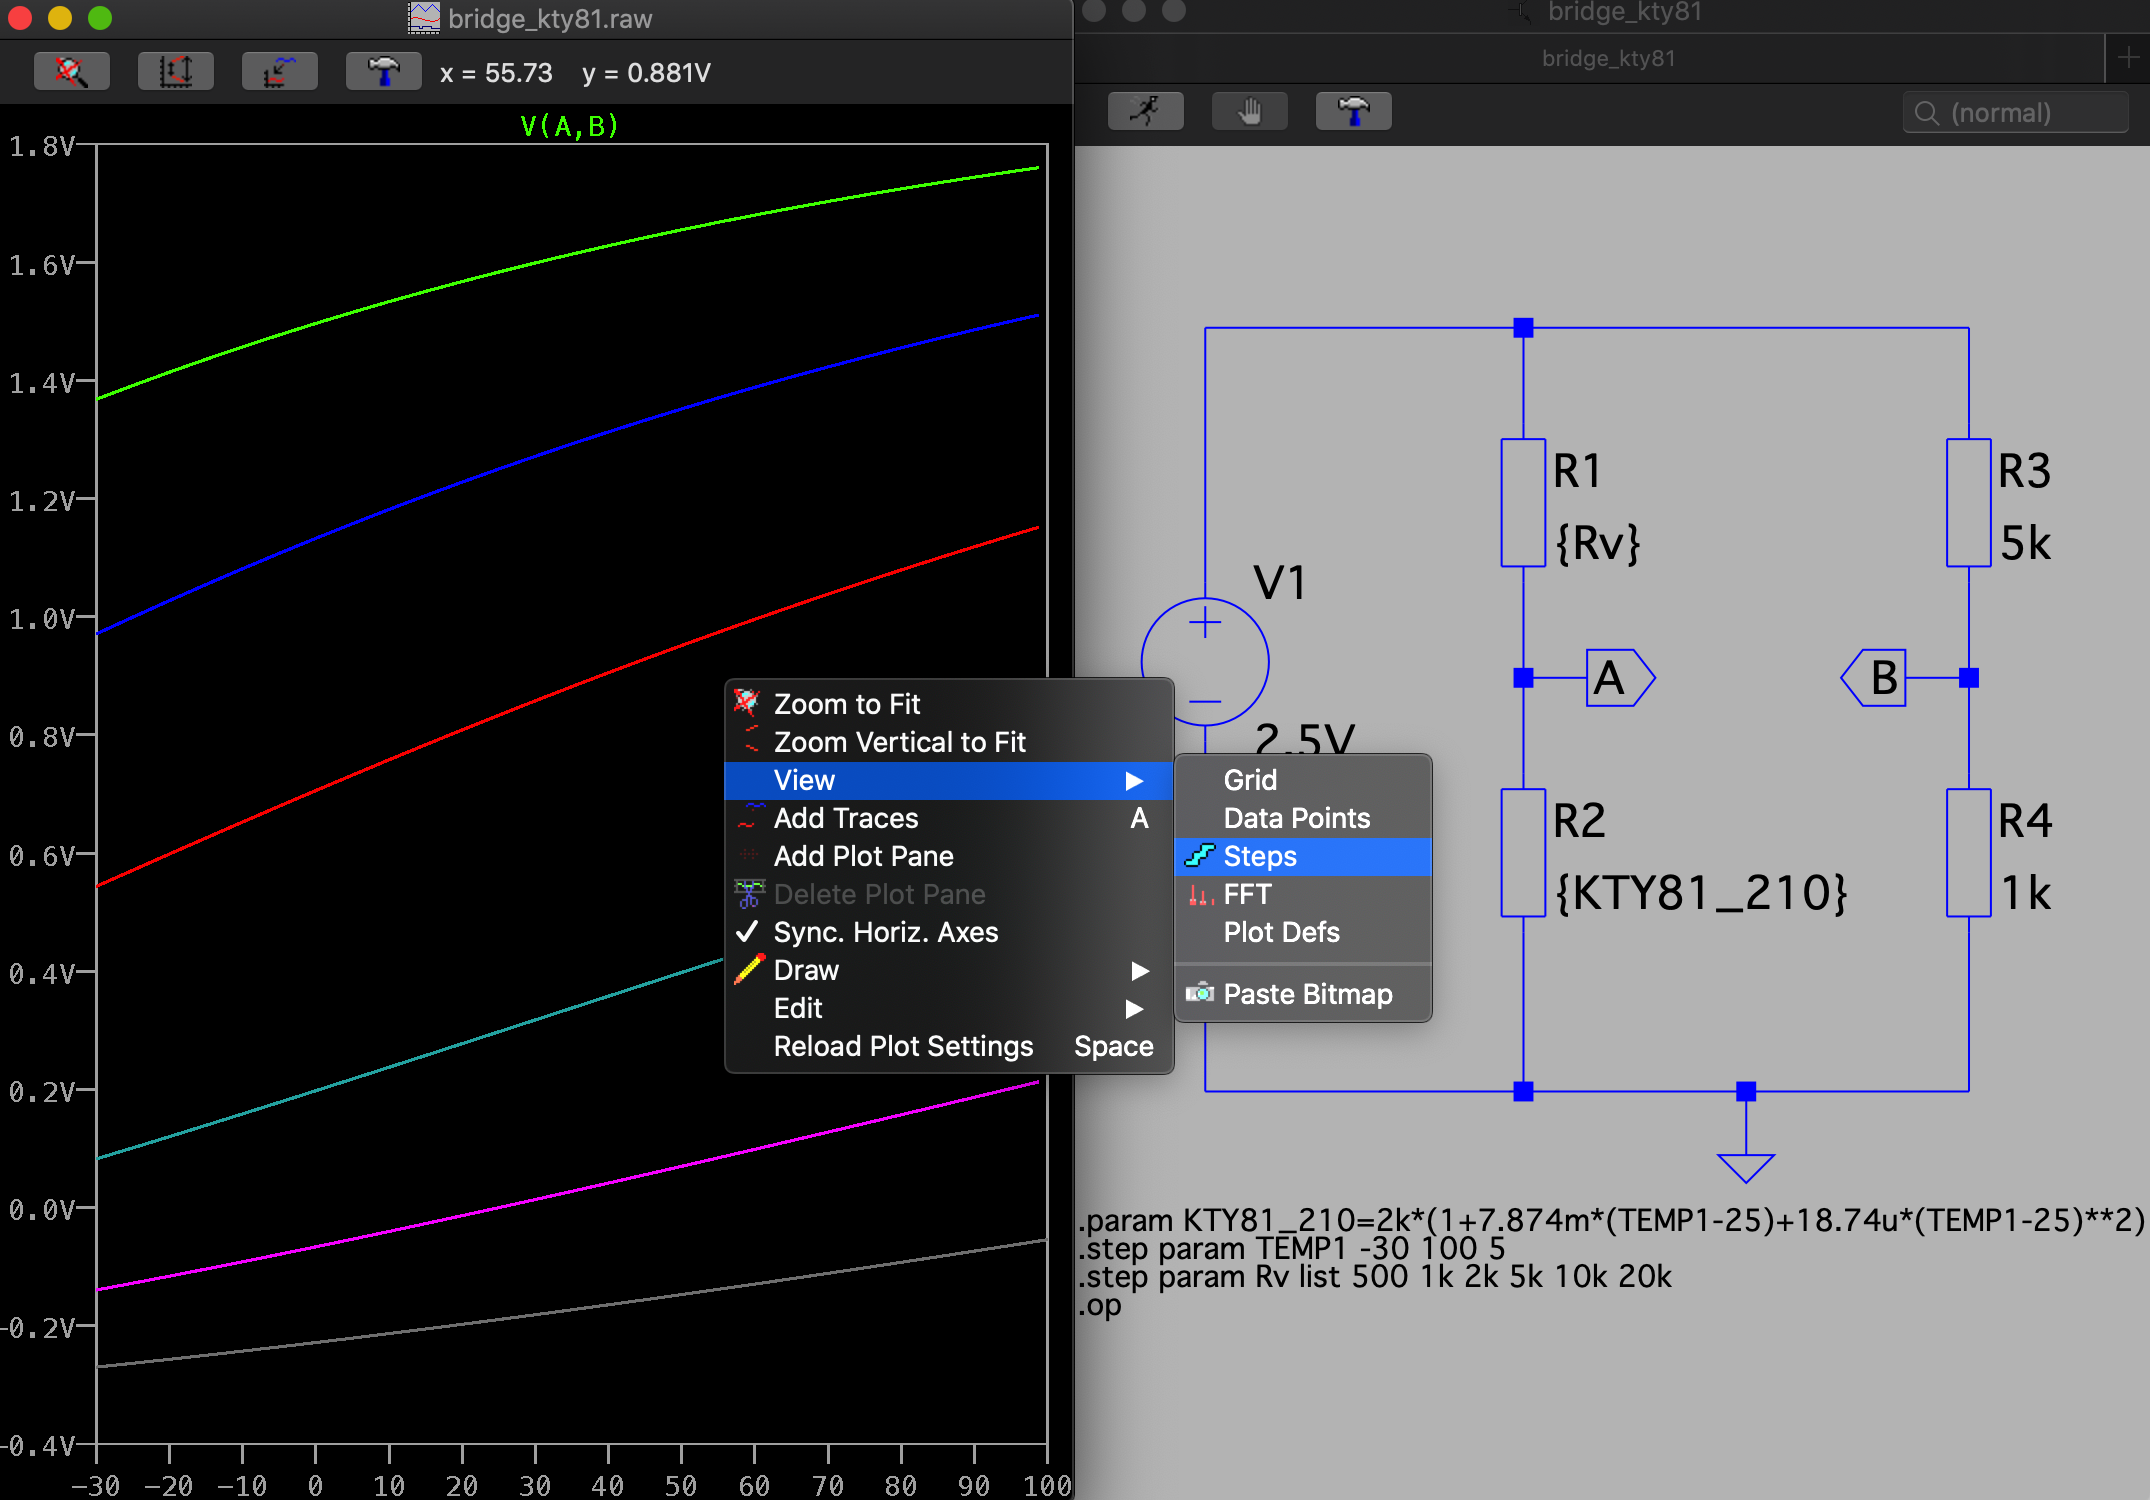
\includegraphics[width=0.95\linewidth]{pictures/mb_kty81_steps.png}
           \end{figure}
       \end{minipage} 
       &
        \begin{minipage}{0.5\textwidth}
            \begin{itemize}
                \item Variiert den Vorwiderstand $R_1$ als Parameter $R_V$
                \item Über die Spice-Direktive $.step\ param\ <Var>\ list\ <Wert_1>\ ...\ <Wert_n>$ könnt ihr eine Liste von Werten hinterlegen
                \item Wir wählen einen Wertebereich von $500\Omega$ - $20k\Omega$
                \item Positioniniert die Spice-Direktive $.step param Rv$ \textbf{nach} der Temperatur $TEMP1$, da der erste Wert auf der Abzisse dargestellt wird
                \item Im waveform viewer könnt ihr über $rechter\ Mausklick$ $->$ $View$ $->$ $Steps$ die einzelnen Werte auswählen und eigenständig bewerten. 
            \end{itemize}
        \end{minipage}   
       \end{tabular}
       \\\\
       \hline
       \textbf{Hinweis zur Simulationsschrittweite} \\
       \hline \\
       \begin{minipage}{\textwidth}
        Wählt die Schrittweite immer möglichst klein, da zu viele Werte die Übersichtlichkeit erschweren!
        \end{minipage}
    \end{tabular}

    \end{table}
     
    \end{tiny} \end{spacing}

\end{frame}

\begin{frame}[t]{Die Messbruecke - Linearisierung der Kennlinie} 
    
    \begin{spacing}{0.9} \begin{tiny}
      \begin{table}[h!]
      \begin{tabular}{p{10cm} }
        \hline
        \textbf{Analytische Herleitung} \\
        \hline \\
        \begin{minipage}{\textwidth}
            Den exakten Wert kann man auch analytisch Herleiten. Dazu schauen wir uns den Spannungsteiler des PTCs genauer an.
        \end{minipage}
        \begin{minipage}{\textwidth}
            \begin{figure}
                \centering    
                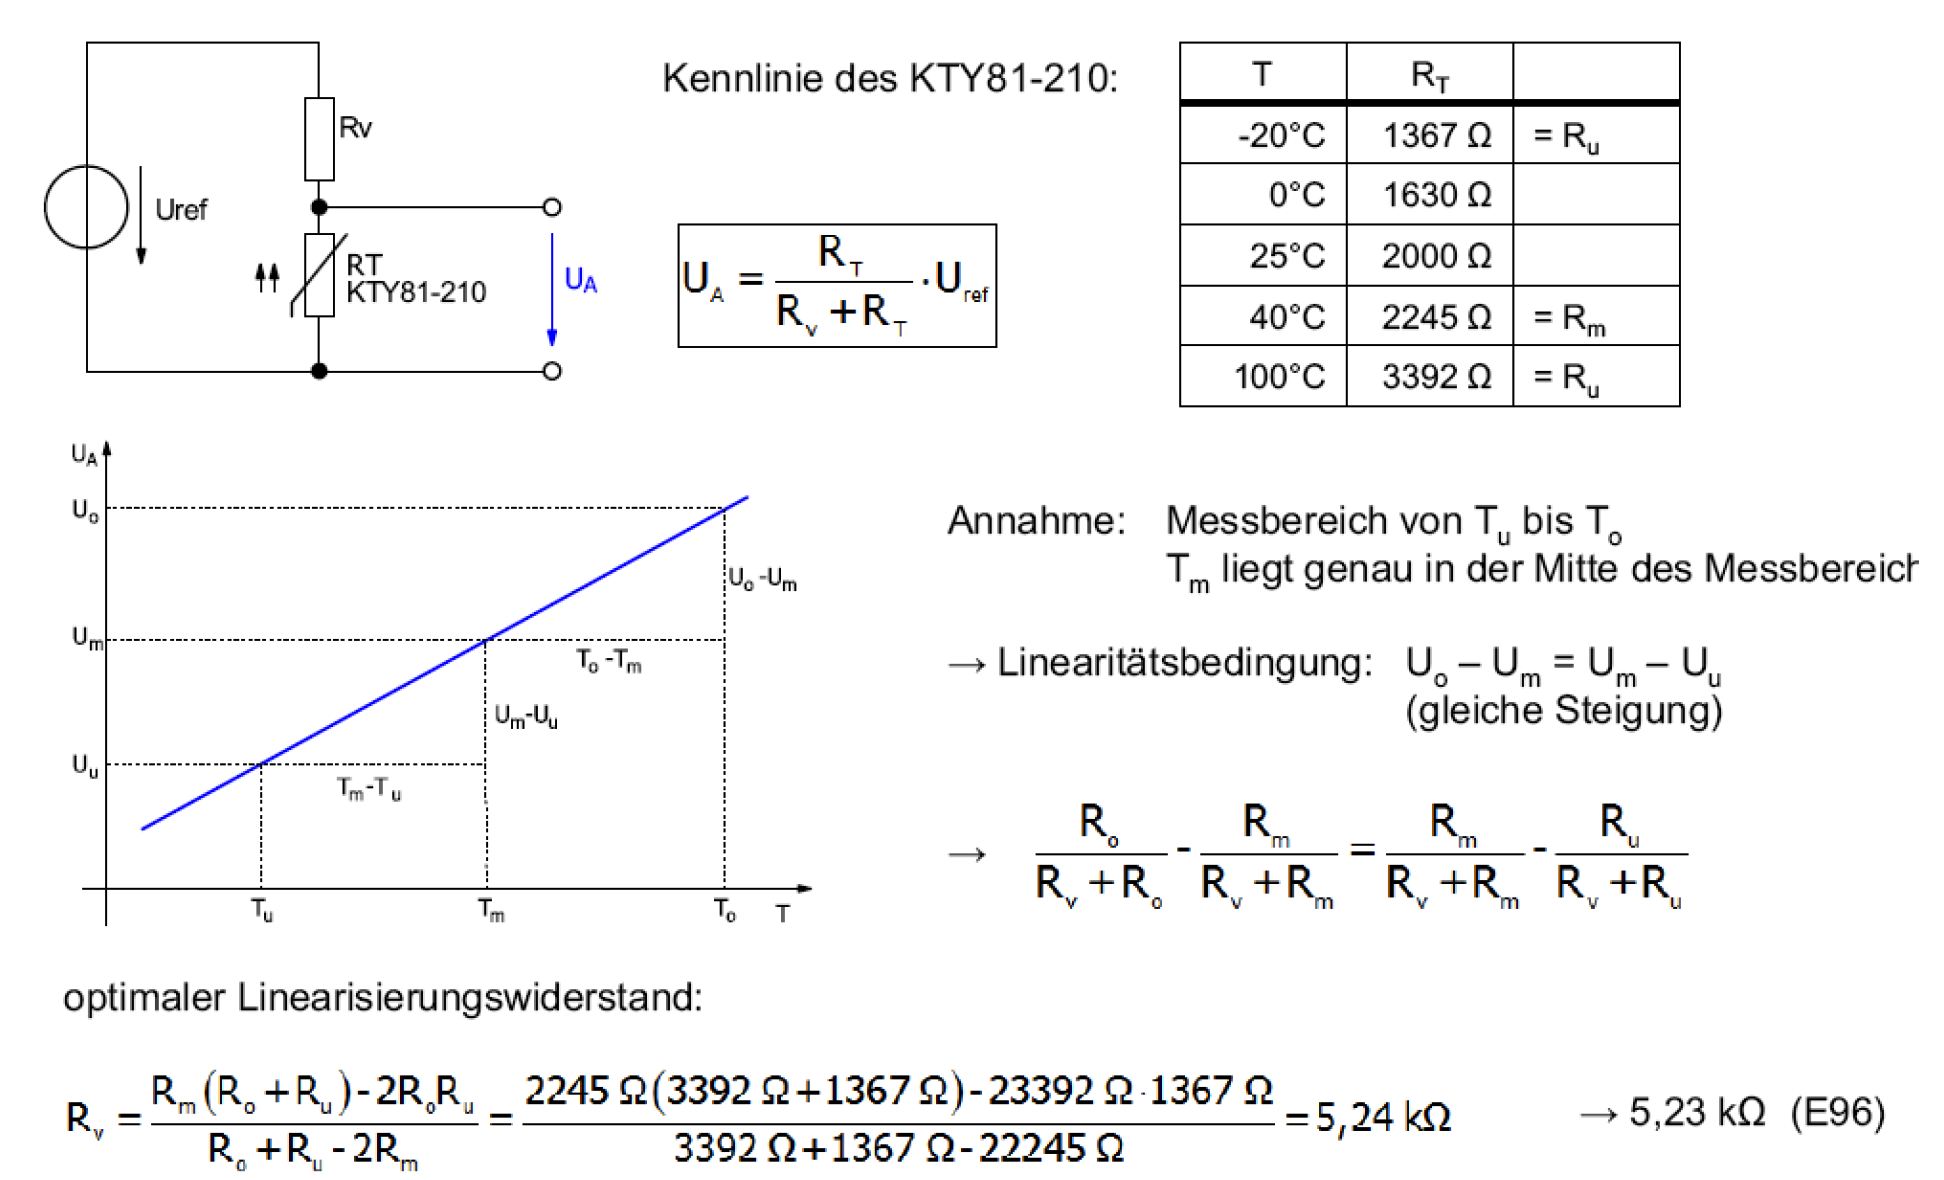
\includegraphics[width=0.9\linewidth]{pictures/linearisierung.png}
            \end{figure}
        \end{minipage}  
       \\        
    \end{tabular}

    \end{table}
     
    \end{tiny} \end{spacing}

\end{frame}